% THIS IS SIGPROC-SP.TEX - VERSION 3.1
% WORKS WITH V3.2SP OF ACM_PROC_ARTICLE-SP.CLS
% APRIL 2009
%
% It is an example file showing how to use the 'acm_proc_article-sp.cls' V3.2SP
% LaTeX2e document class file for Conference Proceedings submissions.
% ----------------------------------------------------------------------------------------------------------------
% This .tex file (and associated .cls V3.2SP) *DOES NOT* produce:
%       1) The Permission Statement
%       2) The Conference (location) Info information
%       3) The Copyright Line with ACM data
%       4) Page numbering
% ---------------------------------------------------------------------------------------------------------------
% It is an example which *does* use the .bib file (from which the .bbl file
% is produced).
% REMEMBER HOWEVER: After having produced the .bbl file,
% and prior to final submission,
% you need to 'insert'  your .bbl file into your source .tex file so as to provide
% ONE 'self-contained' source file.
%
% Questions regarding SIGS should be sent to
% Adrienne Griscti ---> griscti@acm.org
%
% Questions/suggestions regarding the guidelines, .tex and .cls files, etc. to
% Gerald Murray ---> murray@hq.acm.org
%
% For tracking purposes - this is V3.1SP - APRIL 2009

\documentclass{acm_proc_article-sp}

\begin{document}

\title{Casual Analysis of Residual Structural Coverage in Dynamic Symbolic Execution}

%
% You need the command \numberofauthors to handle the 'placement
% and alignment' of the authors beneath the title.
%
% For aesthetic reasons, we recommend 'three authors at a time'
% i.e. three 'name/affiliation blocks' be placed beneath the title.
%
% NOTE: You are NOT restricted in how many 'rows' of
% "name/affiliations" may appear. We just ask that you restrict
% the number of 'columns' to three.
%
% Because of the available 'opening page real-estate'
% we ask you to refrain from putting more than six authors
% (two rows with three columns) beneath the article title.
% More than six makes the first-page appear very cluttered indeed.
%
% Use the \alignauthor commands to handle the names
% and affiliations for an 'aesthetic maximum' of six authors.
% Add names, affiliations, addresses for
% the seventh etc. author(s) as the argument for the
% \additionalauthors command.
% These 'additional authors' will be output/set for you
% without further effort on your part as the last section in
% the body of your article BEFORE References or any Appendices.

\numberofauthors{1} %  in this sample file, there are a *total*
% of EIGHT authors. SIX appear on the 'first-page' (for formatting
% reasons) and the remaining two appear in the \additionalauthors section.
%
\author{
% You can go ahead and credit any number of authors here,
% e.g. one 'row of three' or two rows (consisting of one row of three
% and a second row of one, two or three).
%
% The command \alignauthor (no curly braces needed) should
% precede each author name, affiliation/snail-mail address and
% e-mail address. Additionally, tag each line of
% affiliation/address with \affaddr, and tag the
% e-mail address with \email.
%
% 1st. author
\alignauthor
Xusheng Xiao

% 2nd. author
%\alignauthor
%G.K.M. Tobin\titlenote{The secretary disavows
%any knowledge of this author's actions.}\\
%       \affaddr{Institute for Clarity in Documentation}\\
%       \affaddr{P.O. Box 1212}\\
%       \affaddr{Dublin, Ohio 43017-6221}\\
%       \email{webmaster@marysville-ohio.com}
%}
% There's nothing stopping you putting the seventh, eighth, etc.
% author on the opening page (as the 'third row') but we ask,
% for aesthetic reasons that you place these 'additional authors'
% in the \additional authors block, viz.
% Just remember to make sure that the TOTAL number of authors
% is the number that will appear on the first page PLUS the
% number that will appear in the \additionalauthors section.

\maketitle
\begin{abstract}

Software developers often face
challenges in reusing open source frameworks due to several factors
such as the framework complexity and lack of proper
documentation. In this paper, we propose a code-search-engine-based
approach that detects \Intro{hotspots} in a given framework
by mining code examples gathered from open source repositories available on the web; 
these hotspots are API classes and methods that are frequently reused. 
Hotspots can serve as starting points for developers
in understanding and reusing the given framework. 
Our approach also detects \Intro{coldspots}, which are API classes and methods that are rarely used.
Coldspots serve as caveats for developers as there can 
be difficulties in finding relevant code examples and are generally less exercised
compared to hotspots. We developed a tool, called SpotWeb, for
frameworks or libraries written in Java and used our tool
to detect hotspots and coldspots of eight widely used open source
frameworks. We show the utility of our detected hotspots 
by comparing these hotspots with the API classes reused by a real application
and compare our results with the results of a previous related approach.
\end{abstract}

\section{Introduction}
\label{sec:introduction}

Since the inception of computer science, many programming languages (\emph{e.g.}, Cobol, Fortran, or Java) have been introduced to serve specific requirements\footnote{\url{http://hopl.murdoch.edu.au}}. For example, Cobol is introduced specifically for developing business applications. In general, software companies or open source organizations often release their applications in different languages to survive in competing markets and to address various business requirements such as platform independence. An empirical study~\citep{jones1998estimating} shows that nearly one third applications have multiple versions in different languages. A natural way to implement an application in a different language is to translate from an existing application. For example, Lucene.Net was translated from Java Lucene according to its website\footnote{\url{http://lucene.apache.org/lucene.net/}}. As another example, the NeoDatis object database was also translated form Java to C\# according to its website\footnote{\url{http://wiki.neodatis.org/}}. During translation, one primary goal is to ensure that both applications exhibit the same behavior.

As existing applications typically use API libraries, it is essential to understand API mapping relations of one programming language, referred to as $L_1$, to another language, referred to as $L_2$, when translating applications from $L_1$ to $L_2$. Researchers~\citep{robillard2009makes,thomas2006api} pointed out that it is hard to use API elements, and our previous work~\citep{zhong2010mining} shows that mapping relations between API elements of different languages can also be complicated. In some cases, programmers may fail to find an existing API element that has the same behavior in the other language. For example, Figures~\ref{fig:db4ojava} and \ref{fig:db40net} show two methods implemented in db4o\footnote{\url{http://www.db4o.com}} of its Java version and its C\# version, respectively. When translating the Java code shown in Figure~\ref{fig:db4ojava} to C\#, programmers of db4o may fail to find an existing C\# class that has the same behaviors with the \CodeIn{Byte\-Array\-Input\-Stream} class in Java, so they implement a C\# class with the same name to fix the behavioral difference. Behavioral differences of mapped API elements (\emph{i.e}., classes, methods, and fields of API libraries) may occur in many places. To reduce translation effort, programmers of db4o developed their own translation tool, called Sharpen\footnote{\url{http://developer.db4o.com/Blogs/News/tabid/171/entryid/653/Default.aspx}}, for translating db4o from Java to C\#. For API translation, Sharpen systematically replaces all API elements in Java with equivalent elements in C\# to ensure that translated C\# applications have the same behaviors with the original Java ones.

\begin{figure}[t]
\begin{CodeOut}%\vspace*{-2ex}
\begin{alltt}
01: private long readLong(ByteArrayInputStream is)\{
02:  ...
03:  l += ((long) (is.read())) << i;
04:  ...\}
\end{alltt}
\end{CodeOut}%\vspace*{-4ex}
\caption{A method in the Java version of db4o.}%\vspace*{-2ex}
\label{fig:db4ojava}
\begin{CodeOut}%\vspace*{-2ex}
\begin{alltt}
05: private long ReadLong(ByteArrayInputStream @is)\{
06:  ...
07:  l += ((long)(@is.Read())) << i;
08:  ...\}
\end{alltt}
\end{CodeOut}%\vspace*{-4ex}
\caption{A method in the C\# version of db4o.}%\vspace*{-4ex}
\label{fig:db40net}
\end{figure}

In practice, as pointed out by Keyvan Nayyeri\footnote{\url{http://dotnet.dzone.com/print/26587}}, one of the most common problems is that translated code does not return expected outputs, partially because behavioral differences of mapped API elements are not fully fixed. For example, when JLCA\footnote{JLCA is a Java-to-C\# translation tool developed by Microsoft. The website of JLCA is \url{http://msdn.microsoft.com/en-us/magazine/cc163422.aspx}} translates the \CodeIn{java.lang.String.indexOf(int)} method from Java to C\#, it generates a warning message: ``Method \CodeIn{java.lang.String. indexOf} was converted to \CodeIn{System.String.IndexOf}, which may throw an exception''. Still, the report does not describe where such an exception is thrown or how to deal with that exception. As programmers typically do not know where such behavioral differences occur, it is difficult for programmers to fix such differences in advance, and thus defects can be introduced in translated applications. To prevent those defects, it is desirable to detect behavioral differences between mapped API elements in different languages. However, existing approaches~\citep{orso1using,jin2010automated,jiang2009automatic,lindigaadebug2005} solve different problems, and cannot detect such differences effectively since these existing approaches require that both the versions under consideration belong to the same language. In our context, the versions under consideration belong to different languages, making these existing approaches inapplicable.


To address the preceding issue, we propose a novel approach, called TeMAPI (\textbf{Te}sting \textbf{Ma}pping relations of \textbf{API}s), that generates test cases to detect behavioral differences among API mapping relations automatically. In particular, TeMAPI accepts two inputs: a translation tool under analysis and a test-generation tool for generating test cases. Given a translation tool that translates applications from one language $L_1$ to the other language $L_2$, TeMAPI generates various test cases to detect behavioral differences among the API mapping relations by effectively leveraging the test-generation tool. TeMAPI next executes translated test cases to detect behavioral differences.

TeMAPI addresses four major technical challenges in effectively detecting behavioral differences. (1) It is challenging to directly extract API mapping relations from translation tools. The primary reason is that often translation tools either use different formats for specifying API mapping relations or do not explicitly describe these mapping relations. For example, Java2CSharp\footnote{Java2CSharp is a Java-to-C\# translation tool developed by ILOG (now IBM). The website of Java2CSharp is \url{http://j2cstranslator.sourceforge.net/}} uses mapping files, Sharpen hardcodes relations in source files, and closed source translation tools such as JLCA typically hide mapping relations in binary files. To address this issue and to be independent of the translation tool under analysis, TeMAPI analyzes translated code for extracting those relations. (2) Interfaces of two mapped API elements can be different, and one API element can be translated to multiple API elements. For example, JLCA translates the \CodeIn{java.net.DatagramSocket.receive(DatagramPacket)} method in Java as shown in Figure~\ref{fig:javacode} to multiple C\# elements as shown in Figure~\ref{fig:codeJLCA}.
To address this issue, TeMAPI uses a technique, called wrapper methods (Section~\ref{sec:approach:wrapper}), that abstracts interface differences among mapped API elements and provides a common interface to effectively apply test-generation tools. (3) Using a basic technique such as generating test cases with \CodeIn{null} values may not be significant in detecting behavioral differences among API mapping relations. Since we focus on object-oriented languages such as Java or C\# to detect behavioral differences, generated test cases need to exercise various object states, which can be achieved using method-call sequences. To address this issue, TeMAPI leverages two existing state-of-the-art test-generation techniques: random~\citep{pacheco2007feedback} and dynamic-symbolic-execution-based~\citep{koushik:cute, godefroid:dart, tillmann2008pex} ones. (4) API elements are typically quite large in size, and it is difficult to check all outputs, posing a test oracle barrier. To overcome the barrier, TeMAPI uses return values of wrapper methods or exceptions being thrown as test oracles. We describe more details of our approach to address these challenges in subsequent sections.

In this paper, although we present our approach for detecting behavioral differences among mapping relations of different languages, our approach is general and can be applied to other software engineering problems where an API needs to be replaced with another API without changing the behavior of an application (\emph{e.g.}, library upgrades~\citep{Kawrykow:2009} or migrating from one library to another library~\citep{nita2010using}).

This paper makes the following major contributions:

\begin{itemize}\vspace*{-1ex}
\item A novel approach, called TeMAPI, that automatically generates test cases to detect behavioral differences among API mapping relations. %\vspace*{-1.5ex}
\item A tool implemented for TeMAPI and four evaluations on five popular translation tools. Unlike untranslated code elements, behavioral differences introduce no compilation errors to be detected, and can lead to defects in translated applications silently. Our results show that existing translation tools can translate most lines from Java to C\#, although these tools typically cover a small set of API mapping relations. Our results also show the effectiveness of our approach in detecting behavioral differences of mapped API elements between different languages.
\item The first empirical comparison on behavioral differences of mapped API elements between the J2SE and .NET frameworks. As shown in Section~\ref{sec:evaluation}, the comparison reveals 8 behavioral differences between mapped API elements in existing translation tools. We analyze these findings, and conclude their implications that are valuable to vendors of translation tools for improving their tools, programmers who use translation tools for being aware of such differences in advance, and developers of API libraries for implementing more translatable APIs.
\end{itemize}\vspace*{-1ex}

The rest of this paper is organized as follows.
%Section~\ref{sec:mapping} presents our test adequacy criteria.
Section~\ref{sec:example} presents an illustrative example.
Section~\ref{sec:approach} presents our approach.
Section~\ref{sec:evaluation} presents our evaluation.
Section~\ref{sec:real} presents capabilities of existing translation tools to translate real projects and discusses importance of our major findings.
Section~\ref{sec:discuss} discusses issues of our approach.
Section~\ref{sec:related} presents related work.
Section~\ref{sec:conclusion} concludes.
\begin{figure}[t]
\begin{CodeOut}%\vspace*{-2ex}
\begin{alltt}
09: DatagramSocket socket = ...;
10: DatagramPacket package = ...;
11: socket.receive(package);
\end{alltt}
\end{CodeOut}%\vspace*{-5ex}
\caption{Sample code in Java.}%\vspace*{-2ex}
\label{fig:javacode}
\begin{CodeOut}%\vspace*{-2ex}
\begin{alltt}
12: UdpClient socket = ...;
13: IPEndPoint remoteIpEndPoint = ...;
14: try\{
15:  byte[] data_in = socket.Receive(ref remoteIpEndPoint);
16:  PacketSupport tempPacket =
          new PacketSupport(data_in, data_in.Length);
17:   tempPacket.IPEndPoint = remoteIpEndPoint;
18: \} catch (System.Exception e)\{...\}
19: PacketSupport package = tempPacket;
\end{alltt}
\end{CodeOut}%\vspace*{-5ex}
\caption{Translated C\# code by JLCA.}%\vspace*{-4ex}
\label{fig:codeJLCA}
\end{figure}

%As stated by Sebesta~\citep{sebesta2002concepts}, modern programming languages start around 1958 to 1960 with the development of Algol, Cobol, Fortran and Lisp. Ever since then, thousands of programming languages came to existence as shown by HOPL website\footnote{\url{http://hopl.murdoch.edu.au}}. For various considerations, programmers often need to translate projects from one language to another language. For example, as stated by , to provide the language and platform independence, he translates Compose*~\citep{garcia-compose} in C\# to Compose*/J in Java. To relief the efforts of translating, programmers may use existing translation tools or even implement their own translation tools. For example, Salem \emph{et al.}~\citep{AgtashAEMBS06} report their experience of translating the BLUE financial system of the ICT company from Java to C\# by the JLCA\footnote{\url{http://tinyurl.com/2c4coln}} tool. For another example, to translate db4o\footnote{\url{http://www.db4o.com}} from Java to C\#, its programmers develop their own translation tool named Sharpen\footnote{\url{http://tinyurl.com/22rsnsk}}.

%To translate a source file, a translation tool needs to its structures and its used API elements. As a project typically use thousands of API elements, it is often more difficult to translate used API elements especially for those languages whose structures are similar. In particular, El-Ramly \emph{et al.}~\citep{el2006experiment} conduct an experiment to translate Java programs to C\#. One of their learnt lessons is ``it
%becomes very important to develop methods for
%automatic API transformation''. Barry compares C\# with Java\footnote{\url{http://tinyurl.com/26d8xcp}}, and claims ``although coding in C\# is easy for a Java programmer..., the biggest challenge in moving from Java to the .NET Framework is learning the details of another set of class libraries''. If not knowing API mapping relations, a translation tool or a programmer cannot translate used API elements correctly. Even when such mapping relations are available, a migration process may introduce defects in translated code since mapped API elements can have behavioral differences. As reported by Panesar\footnote{\url{http://tinyurl.com/3xpsdtx}}, even most common methods such as \CodeIn{String.subString(int, int)} can have behavioral differences between Java and C\#. We investigate the mapping relations of existing translation tools, and we confirm that the behavioral differences of mapped API elements can cause defects in translated code. In particular, in Java2CSharp\footnote{\url{http://j2cstranslator.sourceforge.net/}}, one item of mapping files is described in its mapping files as follows:
%
%\begin{CodeOut}%\vspace*{-2ex}
%\begin{alltt}
%1 package java.lang::System\{
%2  class java.lang.String :: System:String\{
%3   method valueOf(Object) { pattern = @1.ToString(); }
%4   ...\}\}
%\end{alltt}
%\end{CodeOut}
%
%Line 2 of this item describes that the \CodeIn{java.lang.String} class in Java is mapped to the \CodeIn{System.String} class in C\#. Line 3 of this item describes that the \CodeIn{java.lang.String.valueOf(Object)} method is mapped to the \CodeIn{System.String.ToString()} method in C\#, and \CodeIn{@1} denotes the first parameter of the \CodeIn{valueOf(Object)} method. Based on the preceding mapping relation, Java2CSharp translates a Java code snippet (Lines 5 and 6) to a C\# code snippet (Lines 7 and 8) as follows.
%
%\begin{CodeOut}%\vspace*{-2ex}
%\begin{alltt}
%\textbf{  Java Code}
%5 Object obj = ...
%6 String value = java.lang.String.valueOf(obj);
%\textbf{  C# Code translated by Java2CSharp}
%7 Object obj = ...
%8 String value = obj.ToString();
%\end{alltt}
%\end{CodeOut}
%
%The translated code snippet compile well, but it has behavioral differences with the original Java code snippet. For example, if Line 5 assigns null to \CodeIn{obj}, \CodeIn{value} of Line 6 will be ``null''. If Line 7 assigns null to \CodeIn{obj}, \CodeIn{value} of Line 8 will not be set to ``null'' since it throws \CodeIn{NullReferenceException}.
%
%As it throw exceptions, the preceding difference of API mapping relation is relatively easy to detect since programmers often use extreme inputs such as null values as test cases. In particular, Sharpen is aware of the differences, and the mapping relation in Sharpen is defined as follows:
%
%\begin{CodeOut}
%\begin{alltt}
%9 public abstract class Configuration \{
%10 protected void setUpStringMappings() \{
%11   mapMethod("java.lang.String.valueOf",
%              runtimeMethod("getStringValueOf"));
%12  ...\} \}
%\end{alltt}
%\end{CodeOut}
%
%Based on Line 11 of the preceding mapping relation, Sharpen translates the Java code snippet (Lines 5 and 6) to a C\# code snippet (Lines 7 and 8) as follows.
%
%\begin{CodeOut}%\vspace*{-2ex}
%\begin{alltt}
%\textbf{  C# Code translated by Sharpen}
%13 Object obj = ...
%14 String value = getStringValueOf(obj);
%\end{alltt}
%\end{CodeOut}
%
%In Sharpen, the \CodeIn{getStringValueOf(object)} method is implemented as follows:
%
%\begin{CodeOut}%\vspace*{-2ex}
%\begin{alltt}
%15 public static string GetStringValueOf(object value)\{
%16  return null == value? "null": value.ToString();
%17	\}
%\end{alltt}
%\end{CodeOut}
%
%If Line 13 assigns a null value to \CodeIn{obj}, \CodeIn{value} in Line 14 will also be ``null'' as expected. By implementing its own mapped C\# method, Sharpen hides the preceding difference, but it still fails to hide all differences. For example, we find that if Line 5 assigns a \CodeIn{false} boolean value to \CodeIn{obj}, \CodeIn{value} in Line 6 will be ``false'', but if Lines 7 and 13 assign a \CodeIn{false} boolean value to \CodeIn{obj}, \CodeIn{value} of Line 8 and \CodeIn{value} in Line 14 will both be ``False''. This difference is relatively difficult to detect, since a programmer typically does not know the internal logic of the method to construct appropriate test cases.
%
%
%It is desirable to detect differences of API mapping relations since the differences will potentially introduce defects to client codek, the same inputs, but it is challenging to detect behavioral differences of API mapping relations via testing for three factors: (1) API elements are typically quite large in size, so it takes great efforts to write test cases manually for API elements and their mapping relations; (2) Other types of migrations such as library migrations~\citep{nita2010using} can use existing test cases to ensure the quality of migrated code, but for language migration, translated test cases may also have defects at the first place; (3) It requires many test cases to reveal all behaviors of API elements, and simply generating extreme values such as null values are not sufficient to reveal all API behaviors.
%
%In this paper, we propose an approach, called TeMAPI (\textbf{Te}sting \textbf{Ma}pping relations of \textbf{API}s), that detects behavioral differences of API mapping relations via testing. TeMAPI generates various test cases and compares testing results of mapped API elements for their behavioral differences. This paper makes the following major contributions:
%
%\begin{itemize}\vspace*{-1.5ex}
%\item A novel approach, called TeMAPI, that detect behavioral differences of mapped API elements via testing. Given a translation tool, TeMAPI detects behavioral differences of its all API mapping relations automatically. It is important to detect these behavioral differences since they can introduce defects in translated code silently.\vspace*{-1.5ex}
%\item Test adequacy criteria proposed for generating sufficient test cases to test API mapping. TeMAPI targets at generating adequate test cases that can reveal all behaviors of API elements to test their mapping relations.\vspace*{-1.5ex}
%\item A tool implemented for TeMAPI and two
%evaluations on ?? projects that include ?? mapping relations from Java to C\#, and ?? mapping relations from C\# to Java. The results show that our tool detects ?? unique defects of mapping relations...
%\end{itemize}\vspace*{-1.5ex}
%
%The rest of this paper is organized as follows.
%Section~\ref{sec:mapping} presents our test adequacy criteria.
%Section~\ref{sec:example} illustrates our approach using an example.
%Section~\ref{sec:approach} presents our approach.
%Section~\ref{sec:evaluation} presents our evaluation results.
%Section~\ref{sec:discuss} discusses issues of our approach.
%Section~\ref{sec:related} presents related work.
%Finally, Section~\ref{sec:conclusion} concludes.

\section{Example}
\label{sec:example}

TeMAPI includes three major steps in detecting behavioral differences among API elements described in mapping relations. We use JLCA (a Java-to-C\# translation tool) as an example translation tool, and the \CodeIn{java.io.ByteArrayInputStream} class in Java as an example API element to illustrate these three steps.

%----------------------------------------------------
\textbf{Translating Synthesized wrappers.} TeMAPI first synthesizes a Java wrapper class for the example class. TeMAPI next uses JLCA to translate the wrapper class to C\#. TeMAPI compares source code of the synthesized wrapper class with the translated wrapper class to extract translatable API elements of the example class. In particular, our example class in Java has five fields, two constructors, and eight methods besides inherited ones\footnote{\url{http://tinyurl.com/2dsgftv}}. A class can have more than one constructor, and a translation tool may not translate all its constructors. Therefore, to address this issue, TeMAPI includes different constructors in its synthesized wrapper methods instead of simply pushing the receiver object as a parameter of wrapper methods. For example, TeMAPI first identifies \CodeIn{ByteArrayInputStream(byte[])} constructor as translatable, and synthesizes the wrapper method for the \CodeIn{skip(long)} method as follows:

\begin{CodeOut}\vspace*{-1ex}
\begin{alltt}
public long testskip24nm(long m0, byte c0[])\{
  ByteArrayInputStream obj = new ByteArrayInputStream(c0);
  return obj.skip(m0);\}
\end{alltt}
\end{CodeOut}\vspace*{-2ex}

TeMAPI next uses JLCA to translate synthesized wrapper methods from Java to C\#. A translation tool typically cannot include mapping relations for all the API elements between two languages, so translated wrapper methods can have compilation errors. TeMAPI parses translated wrapper methods and filters out all methods with compilation errors. For example, below is the translated \CodeIn{testskip- 24nm} method in C\#:
\vspace*{-2ex}

\begin{CodeOut}
\begin{alltt}
public virtual long testskip24nm(long m0, sbyte[] c0)\{
  MemoryStream obj = new MemoryStream(
                    SupportClass.ToByteArray(c0));
  MemoryStream temp_BufferedStream = obj;
  Int64 temp_Int64 = temp_BufferedStream.Position;
  temp_Int64 = temp_BufferedStream.Seek(m0,
       System.IO.SeekOrigin.Current) - temp_Int64;
  return temp_Int64;\}
\end{alltt}
\end{CodeOut}\vspace*{-2ex}

TeMAPI does not remove this method, since it does not result in compilation errors.


\textbf{Generation of C\# Test Cases for Testing Java Code.} A major advantage of our synthesized wrapper is that the original wrapper and the translated wrapper shares the same interface, irrespective of method calls within the wrapper method. Therefore, TeMAPI detects behavioral differences between mapped API elements by generating test cases on one version of wrapper methods and applying those test cases on the other version. In particular, TeMAPI extends Pex~\cite{tillmann2008pex} to generate test cases for each remaining C\# wrapper method. For the example class, Pex attempts to explore all feasible paths among method calls within the wrapper methods and generates inputs and outputs that exercise various paths. Based on the inputs and output generated for each path, TeMAPI generates a Java test case to check whether the original wrapper method return the same values as the translated one. For example, TeMAPI generates the following Java test case based on inputs generated by Pex for one feasible path (in the C\# wrapper method) that throws exceptions.

\begin{CodeOut}\vspace*{-1ex}
\begin{alltt}
public void testskip24nm36()\{
  try\{
     Test_java_io_ByteArrayInputStream obj =
        new Test_java_io_ByteArrayInputStream();
     long m0 = java.lang.Long.valueOf(
                  "2147483648").longValue();
     byte[] c0 = new byte[0];
     obj.testskip24nm(m0,c0);
     Assert.assertTrue(false);
  \}catch(java.lang.Exception e)\{
     Assert.assertTrue(true); \}\}
\end{alltt}
\end{CodeOut}\vspace*{-2ex}

This Java test case fails, since given the preceding inputs, the \CodeIn{skip (long)} method in Java does not throw any exceptions, instead the translated C\# code does. Thus, TeMAPI detects a behavioral difference between the \CodeIn{skip(long)} method in Java and its translated C\# API elements by JLCA.

%-----------------------------------
\textbf{Generation of Java Test Cases for Testing C\# Code.} As shown by Thummalapenta \emph{et al.}~\cite{thummalapenta09:mseqgen}, Pex cannot effectively generate sequences. To address this issue, TeMAPI extends Randoop~\cite{pacheco2007feedback} for testing Java code to generate invocation sequences. TeMAPI does not generate invocation sequences from wrappers directly, since each wrapper method includes a fixed simple invocation sequence. Instead, TeMAPI uses translatable API methods in Step 1, and limits the scope of Randoop to those methods while generating invocation sequences. For example, a generated Java test case is as follows:

\begin{CodeOut}\vspace*{-1ex}
\begin{alltt}
public void test413() throws Throwable\{
  ...
  ByteArrayInputStream var2=new ByteArrayInputStream(...);
  var2.close();
  int var5=var2.available();
  assertTrue(var5 == 1);\}
\end{alltt}
\end{CodeOut}\vspace*{-2ex}


The test case gets passed, since Java allows access to the stream even if the stream is closed. TeMAPI next uses JLCA to translate the generated Java test case from Java to C\#. Since the Java test case uses only translatable API elements, JLCA translates the test case to a C\# test case as follows:

\begin{CodeOut}\vspace*{-1ex}
\begin{alltt}
public void test413() throws Throwable\{
  ...
  MemoryStream var2 = new MemoryStream(...);
  var2.close();
  long available = var2.Length - var2.Position;
  int var5 = (int) available;
  AssertTrue(var5 == 1);\}
\end{alltt}
\end{CodeOut}\vspace*{-2ex}

In contrast to the Java test case, the C\# test case gets failed since C\# does not allow such access to the stream and throws \CodeIn{ObjectDis\\posedException}. TeMAPI thus detects a behavioral difference with invocation sequences.

This example motivates our basic idea of generating test cases in one language and translating those test cases to another language for detecting differences among API mapping relations. %We next present details of our approach.

%\begin{figure}[t]
%\centering %\hfill
%\includegraphics[scale=0.95,clip]{figure/sample.eps}\vspace*{-3ex}
% \caption{\label{fig:example}API mapping}\vspace*{-4ex}
%\end{figure}

%Based on the mapping relations, a translation tool can migrate the
%preceding code snippet automatically. To learn the mapping
%relations,
%
%%\begin{figure}[t]
%%\centering
%%\includegraphics[scale=0.86,clip]{figure/openfile.eps}\vspace*{-1.5ex}
%% \caption
%%{\label{fig:openfile}Aligned wrapper}\vspace*{-2ex}
%%\end{figure}
%
%In this section, we illustrate the main steps of MAM to
%mine the API mapping in Java for \CodeIn{System.IO.Directory.
%Exists()} in C\# from the HypoLog
%project\footnote{\url{http://sourceforge.net/projects/twlog/}}.
%
%The first step of MAM is to align classes and methods of
%wrapper by names. This step finds class pairs and method pairs
%that implement similar functionalities, and each pair may use
%API mapping since it implements a similar functionality. Our
%approach chooses names to align classes and methods because these
%classes and methods are from the same project. In this example, our
%approach aligns the two methods as shown in
%Figure~\ref{fig:openfile} because the two method have similar names
%and their declaring classes also have similar names (see
%Section~\ref{sec:approach:alignclientcode} for details).
%
%The second step of MAM is to mine mapping relations of API
%classes based on the names of corresponding fields, parameters,
%returned types, and local variables. This step also relies on names
%for the same consideration of the first step. For example, our
%approach maps the two parameters with the same name as shown by the
%red arrow of Figure~\ref{fig:openfile}. From the types of the two
%parameters, MAM mines the mapping relation between two API
%classes: \CodeIn{System.String} $\leftrightarrow$
%\CodeIn{java.lang.String} (see
%Section~\ref{sec:approach:mappingtypes} for details).
%
%
%The final step of MAM is to mine mapping relations of API
%methods. Besides the factors listed in
%Section~\ref{sec:introduction}, another factor is that API calls in
%wrapper are often not carefully aligned. To deal with those
%challenges, MAM first builds an API Transformation Graph
%(ATG) for each method. After that, MAM compares built
%graphs to mine mapping relations of API methods (see
%Section~\ref{sec:approach:mappingtypes} and
%Figure~\ref{fig:approach1} for details). Figure~\ref{fig:example}
%shows the mined mapping relation between
%\CodeIn{System.IO.Directory.Exists()} and its API mapping in
%Java.


\bibliographystyle{plain}
\bibliography{mybib}

\end{document}
